\section{Objetivos}

\begin{itemize}
    \item Diseñar, simular e implementar un controlador \textbf{LQR} para un sistema de \textbf{péndulo rotatorio invertido}.
    \item Comparar los resultados de \textbf{simulación} e \textbf{implementación}.
    \item Analizar cómo la variación de las matrices \textbf{Q} y \textbf{R} afecta la respuesta del sistema y el esfuerzo de control.
    \item Explicar el funcionamiento del algoritmo \textbf{swing-up} y su integración con el control de balanceo del péndulo.
\end{itemize}

\section{Hardware y software}
\begin{center}
\renewcommand{\arraystretch}{1.2}
\begin{tabular}{|c|p{0.62\textwidth}|c|}
\hline
\textbf{Nº} & \textbf{Descripción} & \textbf{Cantidad} \\\hline
1 & Módulo QUBE-Servo con péndulo invertido & 1 \\\hline
2 & QUARC para MATLAB/Simulink & 1 \\\hline
\end{tabular}
\end{center}

\section{Péndulo rotatorio invertido de Quanser}

 El sistema está formado por un \textbf{brazo rotatorio actuado} acoplado al eje del \textbf{QUBE-Servo} y un \textbf{péndulo} unido al extremo de dicho brazo. En este modelo, \(\theta\) representa el ángulo del brazo rotatorio, \(\alpha\) el ángulo del péndulo y \(V_m\), el  voltaje aplicado al motor. Las ecuaciones de movimiento del sistema se obtienen mediante el método de \textbf{Euler-Lagrange} y, posteriormente, se linealizan para obtener una representación en \textbf{espacio de estados}. Para este prelaboratorio, el script \texttt{setup\_qube\_rotpen\_lqr.m} implementa esa formulación a partir de los parámetros físicos del sistema y de la dinámica del actuador, construyendo el modelo con el vector de estados y entrada de la forma:
 \begin{equation}
    x=[\theta\;\alpha\;\dot{\theta}\;\dot{\alpha}]^T \qquad u=V_m   
 \end{equation}
  y las matrices \(A\), \(B\), \(C\) y \(D\), las cuales serán utilizadas en el diseño del controlador \textbf{LQR}. La Figura~\ref{fig:qube_servo_pendulo} muestra el módulo \textbf{QUBE-Servo} con el péndulo rotatorio invertido empleado en este laboratorio. Toda la información completa del modelo, su deducción matemática y la descripción detallada de sus variables y ecuaciones se encuentra en el documento \textit{QUBE-Servo State-Space Modeling Workbook.pdf}.

\begin{figure}[H]
    \centering
    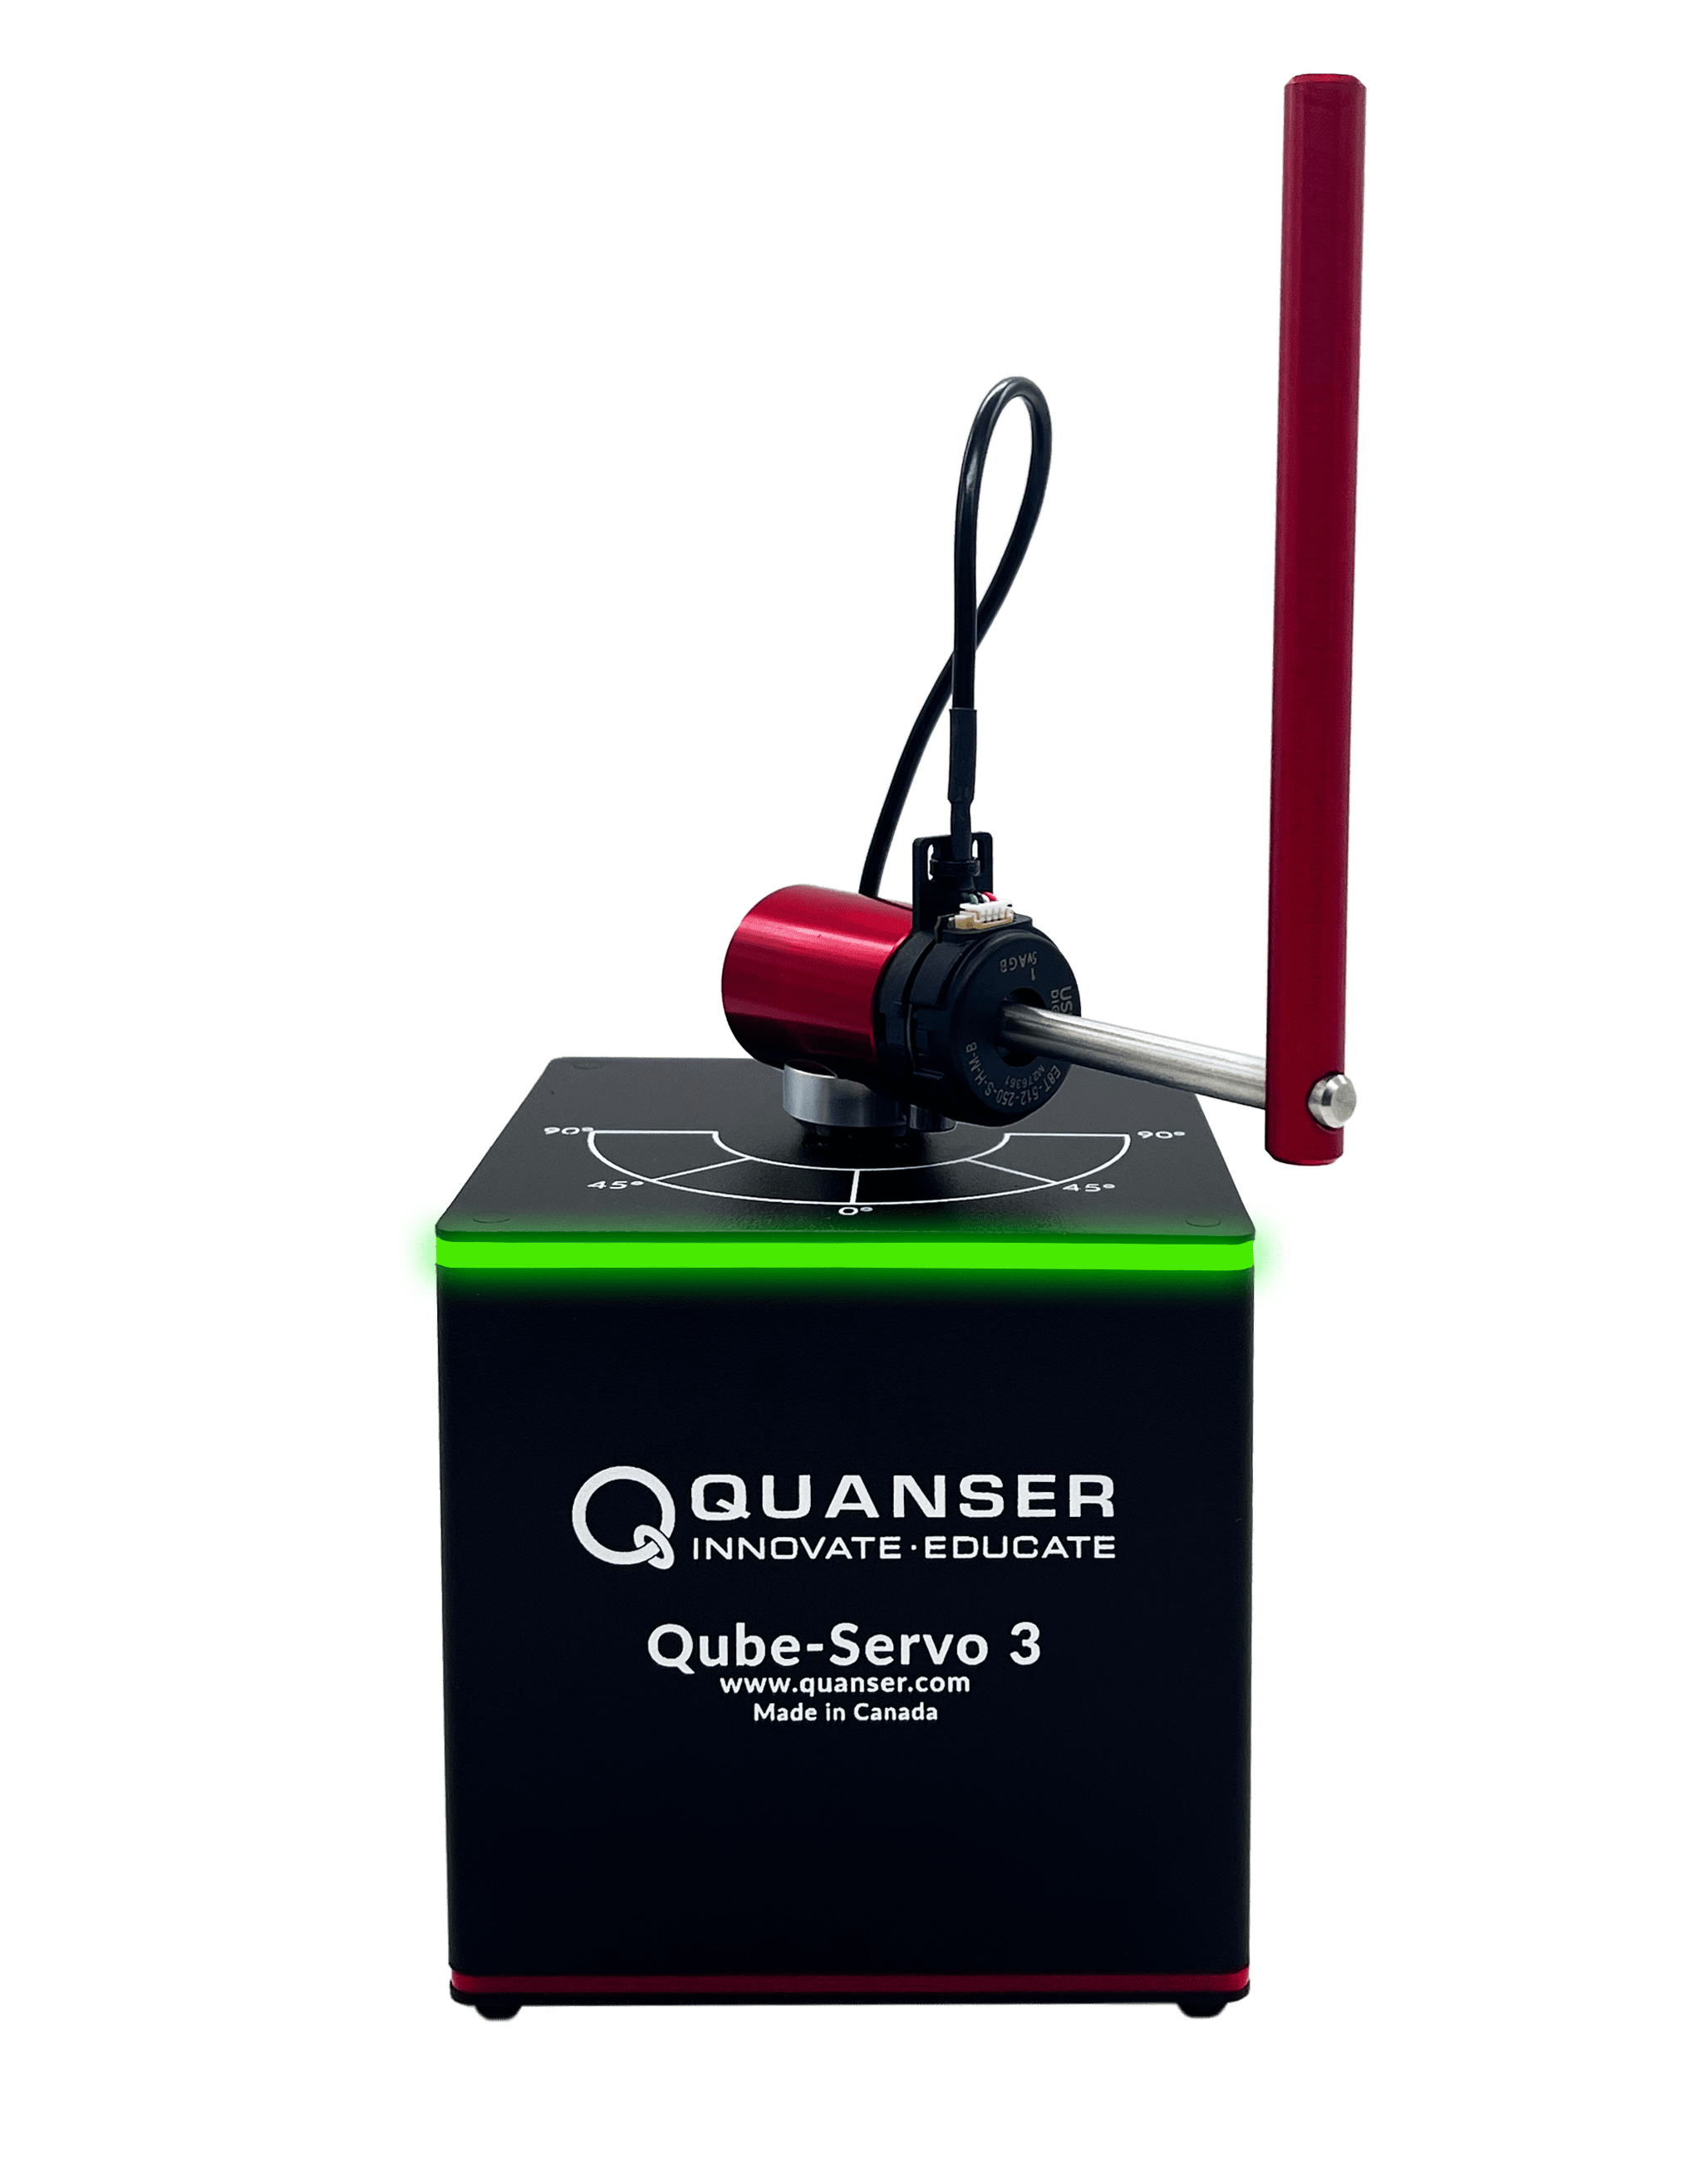
\includegraphics[width=0.42\textwidth]{images/QUBE-Servo3-front-1.png}
    \caption{Módulo QUBE-Servo con péndulo rotatorio invertido.}
    \label{fig:qube_servo_pendulo}
\end{figure}